Given that 
\begin{align}
	\vec{u} = \myvec{-1\\0},\,
	f = -3
\end{align}
Hence, the centre and radius are given as
\begin{align}
	\vec{c} = -\vec{u} = \myvec{1\\0},\,
	r = \sqrt{\norm{\vec{u}}^2 - f}
	  = 2
\end{align}
From \eqref{eq:conic_tangent_qk-circ},
the points of contact for the tangent are given by
\begin{align}
	\label{eq:chapters/12/6/3/19/eq3}
	\vec{q}_{ij} = \brak{\pm r\frac{\vec{n}_j}{\norm{\vec{n}_j}}-\vec{u}} \text{ i,j} = 1,2
\end{align}
Since, tangents are parallel to the x-axis, the normal is given as
\begin{align}
	\vec{n} = \myvec{0\\1}
\end{align}
Substituting in \eqref{eq:chapters/12/6/3/19/eq3} we get
\begin{align}
	\vec{q}_{11} &= \brak{\pm 2\myvec{0\\1} - \myvec{-1\\0}}\\
	&= \myvec{1\\-2},\myvec{1\\2}
\end{align}
Hence, the two points of contact are
\begin{align}
	\myvec{1\\2} \text{ and } \myvec{1\\-2}
\end{align}
See \figref{fig:chapters/12/6/3/19/Fig1}.
\begin{figure}[H]
	\begin{center} 
	    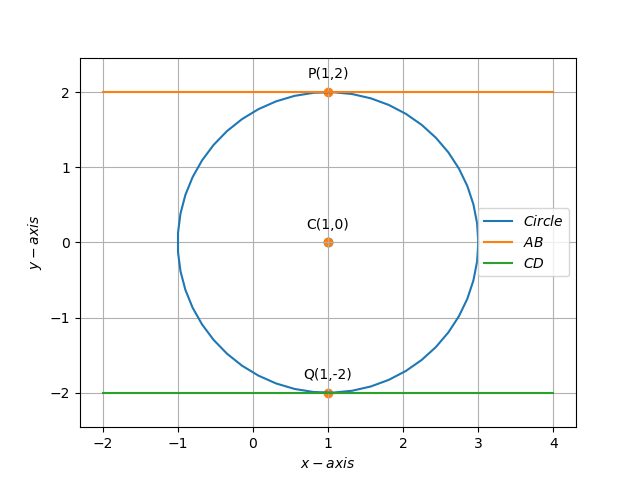
\includegraphics[width=0.75\columnwidth]{chapters/12/6/3/19/figs/tan1}
	\end{center}
\caption{}
\label{fig:chapters/12/6/3/19/Fig1}
\end{figure}





















